%-------------------------------------------------------------------------------
%	PACKAGES AND OTHER DOCUMENT CONFIGURATIONS
%-------------------------------------------------------------------------------

%------------------------------------------------
% BASIC CLASS FILE
%------------------------------------------------

\documentclass{pnastwo}

%------------------------------------------------
% POSITION OF TEXT
%------------------------------------------------

%% Changing position of text on physical page:
%% Since not all printers position
%% the printed page in the same place on the physical page,
%% you can change the position yourself here, if you need to:

% \advance\voffset -.5in % Minus dimension will raise the printed page on the 
                         %  physical page; positive dimension will lower it.

%% You may set the dimension to the size that you need.

%------------------------------------------------
% GRAPHICS STYLE FILE
%------------------------------------------------

%% Requires graphics style file (graphicx.sty), used for inserting
%% .eps/image files into LaTeX articles.
%% Note that inclusion of .eps files is for your reference only;
%% when submitting to PNAS please submit figures separately.

%% Type into the square brackets the name of the driver program 
%% that you are using. If you don't know, try dvips, which is the
%% most common PC driver, or textures for the Mac. These are the options:

% [dvips], [xdvi], [dvipdf], [dvipdfm], [dvipdfmx], [pdftex], [dvipsone],
% [dviwindo], [emtex], [dviwin], [pctexps], [pctexwin], [pctexhp], [pctex32],
% [truetex], [tcidvi], [vtex], [oztex], [textures], [xetex]

\usepackage{graphicx}
\usepackage{tabularx}

%------------------------------------------------
% OPTIONAL POSTSCRIPT FONT FILES
%------------------------------------------------

%% PostScript font files: You may need to edit the PNASoneF.sty
%% or PNAStwoF.sty file to make the font names match those on your system. 
%% Alternatively, you can leave the font style file commands commented out
%% and typeset your article using the default Computer Modern 
%% fonts (recommended). If accepted, your article will be typeset
%% at PNAS using PostScript fonts.

% Choose PNASoneF for one column; PNAStwoF for two column:
%\usepackage{PNASoneF}
%\usepackage{pnastwof}

%------------------------------------------------
% ADDITIONAL OPTIONAL STYLE FILES
%------------------------------------------------

%% The AMS math files are commonly used to gain access to useful features
%% like extended math fonts and math commands.

\usepackage{amssymb,amsfonts,amsmath}

%------------------------------------------------
% OPTIONAL MACRO FILES
%------------------------------------------------

%% Insert self-defined macros here.
%% \newcommand definitions are recommended; \def definitions are supported

%\newcommand{\mfrac}[2]{\frac{\displaystyle #1}{\displaystyle #2}}
%\def\s{\sigma}

%------------------------------------------------
% DO NOT EDIT THIS SECTION
%------------------------------------------------

\begin{document}

%-------------------------------------------------------------------------------
%	TITLE AND AUTHORS
%-------------------------------------------------------------------------------

\title{Context-based configuration management: \linebreak
    state of the art and challenges}

%------------------------------------------------

\author{Ghislain Loaec\affil{1}{University of Burgundy}}

\contributor{Draft}

%-------------------------------------------------------------------------------

\setcounter{secnumdepth}{3}
\maketitle % The \maketitle command is necessary to build the title page

\begin{article}

%-------------------------------------------------------------------------------
%	ABSTRACT, KEYWORDS AND ABBREVIATIONS
%-------------------------------------------------------------------------------

\begin{abstract}
The fundamental objective of ubiquitous computing is to ease the human labor in
computer use.  This results in enhancing the resources available throughout the
physical environment.  In order to extract the maximum benefit of a digital
environment, embeded systems and services must cooperate.  Every single operand
has its own information, merged to circumstances in which a task is performed
gives a context (TODO: Reformulate) The primary challenge with context-handling
interacting with humans, is that there is no standard, reusable model that can
be used to handle context.
\end{abstract}

%------------------------------------------------

\keywords{Context-Aware | Configuration Management}

%------------------------------------------------

\abbreviations{
  CAD, context-aware deployment;
  OMG, object management group;
  CCM, COBRA commponent model;
}

%-------------------------------------------------------------------------------
%	PUBLICATION CONTENT
%-------------------------------------------------------------------------------

\section{Introduction}

\dropcap{C}ontext-aware management introduces on conflicts notion of policy.  A
context-aware system must be capable of mimicking a human’s ability to recognise
and exploit implicit information in the environment, in order to advance the
operations of its functionalities.  Although identifying and deducing a human
activity is a challenge, it is critical that context-aware applications should
operate by conveying the appropriate information to the right place at the right
time through inferring the user’s intention.  Context-aware computing is a
computing paradigm in which applications can discover and take advantage of
contextual information such as location, time of day, people and devices, and
user activity. Context-aware computing is especially suited to the areas of
mobile and pervasive computing. Instead of adapting systems and applications so
that mobility is hidden, context-aware computing provides support for
mobile-aware applications.“

\section{Background}

Definition of context (Much debate has occured and are still takinh place about
the meaning of both context and context aware computing)

\begin{quotation}
  ... any information the can be used to charaterize the situation of an entity.
  An entity is a person, place or object that is considered relevant to the
  interation between a user and an application, including the user and the
  application themselves.  \cite{Abowd1997}
\end{quotation}

- Talk about the ``five W's'' - Comparison with human interactions : use of the
implicit information about the situation, i.e. context, to enhance the
convesational bandwidth.


\begin{quotation}
  Context-aware computing : exploit the progress in sensing and mechanisms for
  observing the environement to systematically collect implict context
  \cite{Abowd2002}
\end{quotation}

Context information can be formed into an abstract model of all actors in a
system.

\begin{quotation}
  Context-aware computing is any system that "adapts according to its location
  of use, the collection of nearby people and objects, as well as changes over
  time" \cite{Schilit1994}
\end{quotation}

\section{Context overview}

\begin{quotation}
  Context is effective only when shared \cite{Winograd2001}. 
\end{quotation}

To ensure context is shared, context must first be gathered and managed by a
context-aware system.  This implies that the context-aware system must
understand what context is before it can go on seeking and categorising this
information. 

\subsection{Classes of context}

Schilit et. al. propose the following classification of context information:
\cite{Schilit1994}

\begin{itemize}
  \item \textbf{Computing Context} - network connectivity, bandwidth, and nearby
          resources such as printers, displays, or workstations.
  \item \textbf{User Context} - the user’s profile, location, nearby people, and
          current social situation. 
  \item \textbf{Physical Context} - lighting, noise level, traffic conditions,
          temperature.
\end{itemize}

Each of these categories contains a wealth of information relevant to the
context-aware system.  They cannot however be used in isolation to full effect.
The intention of the context-aware system is to gather and merge them together
in order to achieve an overall picture of the situation.  After the context is
stored in a buffer or repository, the system will decide then what is relevant
to the user at the present moment.

Context information may alternatively be subdivided into two categories:
physical context and virtual context.

\subsubsection{Virtual context}

The virtual context may include the version of the operating system, the
interface capabilities, the wireless technology used to accomplish
communication, email messages sent and received, and documents edited. 

\subsubsection{Physical context}

The physical context on the other hand may be the presence of another entity, be
it a user or device, the proximity to a particular printer, information
indicating if the user is standing, walking or sitting or the current weather
conditions. This entity can be summarized as any acquirable data by the use of a
sensor : lighting, noise level, traffic conditions, temperature (cf. 3.6)

\subsubsection{Historical context}

The contexts stored accross a time span. Considered to be useful but rarely
used except for mobile applications. The system must decide what historical
information is worthy of being kept. The evaluation the historical information
is prohibitively costly and so requires very efficient algorithms 

\subsection{Context information characterisics}

Researchers at the University of Queensland have classified four
characteristics: (Candolin  Kari 2002)

\begin{enumerate}
    \item \textbf{Context information exhibits a range of temporal
            characteristics}

            Context has already been subdivided into physical and virtual
            environement ; it can be furthermore categorized into :

            \begin{itemize}
                \item Static information : any information related to the user's
                        environement that is invariant.
                \item Dynamic information : must be accumulated continuously,
                        frequently and automatically.
            \end{itemize}

            Additionally, past context information may be needed to understand
            the full state of the environment

    \item \textbf{Context information is imperfect}

            This considers the validity of context, in particular dynamic
            context information.  The speed at which the context information
            changes raises reasons for the doubt over the soundness of the
            context.  This "delay between the production and use of context
            information" \cite{Candolin2002} is a concern.  Other sources of
            concern regarding the soundness of context information include the
            reliability of information context producers : sensor failure,
            broken path between producers or any source that would provide wrong
            or outdated information.

    \item \textbf{Information has many alternative representations}

            The raw data gathered from both physical and virtual environment can
            take on many forms and must be processed when combined with other
            context information.  The probability of the context-aware system
            obtaining a 100\% success rate in "capturing the relationships that
            exist between the alternative representations"
            \cite{Candolin2002} of the context information and the one apt
            to the current situation is extremely low.

    \item \textbf{Context information is highly interrelated}

            Context information derived from a particular origin may have a very
            close link with its source, so much so that it is dependant on the
            origin. 
            Context may not be reliable
            “where the characteristics of the derived information are intimately
            linked to the properties of the information it is derived from”
            \cite{Candolin2002}.

\end{enumerate}

\subsection{Context-aware system}

A context-aware system is characterized by the capability of mimicking the
human's ability to recognise the implicit information in the environment and to
exploit it in order to advance the operations of its functionalities.
Although identifying and deducing a human activity is a challenge.
In terms of configuration management, this results in conveying the appropriate
information to the right place and at the right time through inferring the
user’s intention.
To accomplish this objective, thes context aware system must :

\begin{itemize}
    \item Gather the information
    \item Serialize this information
    \item Merge the information to generate higher context
    \item Automatically take action based on the retrieved information
    \item Make the information available to the user, immediately, in the future,
            or when it is required to enhance and aid in he completion if the
            user's task.
\end{itemize}

The researchers of the Context Toolkit at the University of Berkeley propose
that there are three features that a context-aware application must support:
\cite{Dey2000} 

\begin{enumerate}
    \item Presentation of information and services to a user 
    \item Automatic execution of a service for a user 
    \item Tagging of context to information to support later retrieval
\end{enumerate}

The developers of Kimura System have designed distributed components of a
pervasive context-aware system. These components fall into three classes (Voida
et al 2002), these are: 

\begin{enumerate}
    \item Context Acquisition - the system gathers context information and adds
            it to a repository. 
    \item Context Interpretation - the system converts the gathered context
            information into a working context.
    \item User Interaction, the system displays the working context to the user
\end{enumerate}

\subsection{Gathering context information}

Some context information is explicitly given to the system, such as user's
name, age, email, environement variables or regirstry. Other primitive physical
information such as light, heat, pressure readings can be aquired through the
use of sensors

Location and identity are the most frequently sensed pieces of context. 

\begin{quotation}
Sensors are not always 100\% accurate or reliable, particularly if they are
disposable. The information gathering system must be tolerant of sensor failure,
and any information gathered from sensors must be subjected to sanity checks to
help verify its correctness. Sensor fusion is one method of avoiding this
difficulty \cite{Schmidt1999}
\end{quotation}

Let's take for instance a power plant, with several sensor which gives the
context information of temperature. The system must take some descision wether
to cool generously the reactor or not. The consequences of an
underestimation of the temperature would be catastrophic. It might be prudent
either to simply average the results and  discard reported values
that differ too greatly from what other sensors report. This method would avoid
drastic measures being taken by the context system to correct what it considers
to be temperature variations but are actually simply the result of sensor
failure. 

\subsection{Retrieving context information}

\begin{itemize}
  \item Push Model - The context source gather the context information before it
          is needed. It gives better performances but requires large and frequent
          resource consumption for some information the may never be exploited.
  \item Pull Model - Collects only the context information that is required
          It allows to get the information on demand but is exposed to network
          delays and services unavailability
\end{itemize}

The method of context-data acquisition is very important when designing
context-aware systems because it predefines the architectural style of the
system at least to some extent. Chen (2004) presents three different approaches
on how to acquire contextual information.

\subsubsection{Direct sensor access}

This approach is often used in devices with sensors locally built in. The client
software gathers the desired information directly from these sensors, i.e.,
there is no additional layer for gaining and processing sensor data. Drivers for
the sensors are hardwired into the application, so this tightly coupled method
is usable only in rare cases. Therefore, it is not suited for distributed
systems.

\subsubsection{Middleware infrastrucure}
 
The middleware based approach introduces a layered architecture to context-aware
systems with the intention of hiding low-level sensing details.
This approach is equivalent to client-server model, more flexible the widget
since it promotes the independence of each components in the context-aware
system. Every component must be able to perform the following functionnalities :
establishing connections, organising input and output messages and managing
faults.  This model is significantly more complex but the approach is pretty
straightforward since it supports large range of device and application using
standard coding and networking protocols.

\subsubsection{Context server}

This distributed approach extends the middleware based architecture by
introducing an access managing remote component. Gathering sensor data is moved
to this so-called context server to facilitate concurrent multiple access

\subsection{Achitectures for Managing Context}

Winograd (2001) describes three different context management models for
coordinating multiple processes and components:

\begin{itemize}
        \item \textbf{Widgets}
                The key objective of the widget is to seperate the application
                from the context aquisition issues in order to abstract the
                complexity of collecting and managind the context information.
                The widget is used as a mediator to pass only the pertinent
                information to the application, A context widget functions
                independently of applications, which permits multiple
                applications to use it simultaneously. A context widget is also
                responsible for maintaining a complete history of the context
                aquiered for the user's situation.  It remains the most
                prevalent model.

        \item \textbf{Network services}
                This more flexible approach, argued for example in Hong and
                Landay (2001), resembles the context server architecture.
                Instead of a global widget manager discovery techniques are used
                to find networked services. This service based approach is not
                as efficient as a widget architecture due to complex network
                based components but provides robustness.

        \item \textbf{Blackboard}
                In contrast to the process-centric view of the widget and the
                service-oriented model, the blackboard model represents a
                data-centric view The blackboard model adopts a data-centric
                point of view, matching a specified patterns in data. In this
                asymmetric approach processes post messages to a shared media,
                the so-called blackboard, and subscribe to it to be notified
                when some specified event occurs. Advantages of this model are
                the simplicity of adding new context sources and the easy
                configuration.
\end{itemize}

\subsubsection{Trade-off criteria}

When deciding on the most suitable model for a context aware system, we want to
consider the trade-off characteristics : 

          \begin{itemize}
            \item Efficiency : accelerate the throughput of information
                    considering the the bandwidth and latency caused by the
                    explosion in the number of networked applications and
                    devices.
            \item Effort in configuring : considering te various amount of
                    components, perform a change in the configuration
                    state, without the disruption or total failure of the
                    system, it not a tedious task. This model must make
                    sure the edit is safe.
            \item Robustness : the degree to which the system can cope with
                    failure
            \item Simplicity : 
                    \begin{quotation}
                      a system that requires complex understanding by system
                      builders in order to make use of its facilities will be
                      used only by those who have the dedication and motivation
                      to master it.  \cite{Winograd2001}
                    \end{quotation}
            \item Extensibility : 
                    \begin{quotation}
                      services supporting a general notion of context must be
                      easily extensible to accommodate new and unanticipated
                      sources of context information.  \cite{Ebling2002}
                    \end{quotation}
          \end{itemize}

The trade-offs can be used to compare and contrast the different models for
context management. 

\begin{quotation}
        The widget model has tight coupling of system components, which may make
        it the most efficient model in some circumstances, however it suffers
        from complex configuration and issues with powerlessness in the cause of
        failure. The infrastructure model with its independent components may be
        extremely complex, which is a no factor for many developers, however its
        positive criteria of straightforward configuration and robustness may
        compensate for the negative implication of complexity. Finally the
        blackboard model with its very loosely coupled components may suffer
        from efficiency problems, but it is a simple, robust, easily
        configurable model. \cite{Winograd2001}
\end{quotation}

\subsection{Representing Context}

There are several ways to modelize context information :

\begin{itemize}
    \item Key-Value : simplest data structure for context modelling. They are
            frequently used in various service frameworks, where the key-value
            pairs are used to describe the capabilities of a service
    \item Markup scheme : hierarchical data structure consisting of markup tags
            with attributes and content. Profiles represent typical
            markup-scheme models.
    \item Graphical : Unified Modelling Language (UML), extension to the
            Object-Role Modelling (ORM) by context
    \item Object oriented : use the full power of object orientation (e.g.,
            encapsulation, reusability, inheritance). Existing approaches use
            various objects to represent different context types (such as
            temperature, location, etc.), and encapsulate the details of context
            processing and representation
    \item Logic based : high degree of formality. Typically, facts, expressions
            and rules are used to define a context model. A logic based system
            is then used to manage the aforementioned
    \item Ontology based : represent a description of the concepts and
            relationships. very promising instrument for modelling contextual
            information due to their high and formal expressiveness and the
            possibilities for applying ontology reasoning techniques
\end{itemize}

Conclusion of the evaluation presented in Strang and Linnhoff-Popien
\cite{Strang2004}, based on six requirements, show that ontologies are the most
expressive models and fulfil most of their requirements.

Korpipää et al. \cite{Korpipaa2003} present some requirements and goals having
designed a context ontology:

\begin{itemize}
    \item Simplicity: the used expressions and relations should be as simple as
            possible to simplify the work of applications developers
    \item Flexibility and extensibility: the ontology should support the simple
            addition of new context elements and relations
    \item Genericity: the ontology should not be limited to special kind of
            context atoms but rather support different types of context
    \item Expressiveness: the ontology should allow to describe as much context
            states as possible in arbitrary detail.
\end{itemize}

A single context atom can be described with a couple of attributes. The two most
obvious are:

\begin{itemize}
        \item Context type : category of context such temperature, time, speed,
                etc. This type information may be used as a parameter for a
                context query or a subscription.
        \item Context value : raw data gathered by a sensor. The unit depends on
                the context type and the applied sensor, e.g., degree Celsius,
                miles per hour, MegaByte etc.
\end{itemize}

Context type and context value are not enough information to build a working
context-aware system. Additional attributes that might be useful include:

\begin{itemize}
        \item Time stamp : date/time-value describing when the context was
                sensed. It is needed e.g., to create a context history and deal
                with sensing conflicts.
        \item Source : how the information was gathered. In case of a hardware
                sensor it might hold the ID of the sensor and allow an
                application to prefer data from this sensor.
        \item Confidence : the uncertainty of this context type. Not every data
                source delivers accurate information, e.g., location data
                suffers inaccuracy depending on the used tracking tool
\end{itemize}

\subsection{Interpreting the context}

\begin{quotation}
        Interpretation refers to the the process of raising the level of
        abstraction of a piece of context
        \cite{Dey2001}
\end{quotation}

Approaches :

use context fusion to convert the lower level context into higher level usable
by applications. \cite{Dustdar2007}

\subsection{Layered conceptual framework}

\begin{itemize}
        \item Application
        \item Storage management
        \item Preprocessing : 
                \begin{itemize}
                        \item Translation : not implemented in every
                                context-aware system but may offer useful
                                information if the raw data are too coarse
                                grained. The preprocessing layer is responsible
                                for reasoning and interpreting contextual
                                information
                        \item Aggregation / Composition : consisting of several
                                different context data sources, the single
                                context atoms can be combined to high-level
                                information in this layer 
                \end{itemize}
        \item Raw data retrieval :
                appropriate drivers for physical sensors and APIs for virtual
                and logical sensors. The query functionality is often
                implemented in reusable software components which make low-level
                details of hardware access transparent by providing more
                abstract methods such as getPosition().
        \item Sensors :
                \begin{itemize}
                        \item Physical sensors : hardware sensor to capture
                                physical data
                                \begin{itemize}
                                        \item Light
                                        \item Visual context
                                        \item Audio
                                        \item Motion / acceleration
                                        \item Location
                                        \item Touch
                                        \item Temparature
                                        \item Physical Attributes
                                \end{itemize}
                        \item Virtual sensors : source context data from
                                software applications or services tracking
                                systems, electronic calendar, travel-booking
                                system, mouse mouvement, etc.
                        \item Logical sensors : physical + virtual + additional
                                information from databases in order to solve
                                higher tasks
                \end{itemize}
\end{itemize}

\subsection{Security and Privacy}

As context may include sensitive information on people, e.g., their location and
their activity, it is necessary to have the opportunity to protect privacy. For
these purposes the Context Toolkit introduces the concept of context ownership.
Users are assigned to sensed context data as their respective owners. They are
allowed to control the other users’ access. New components involved in this
access control are the Mediated Widgets, Owner Permissions, a modified
BaseObject and Authenticators. The MediatedWidget class is an extension of a
basic widget which contains a so-called widget developer specifying who owns the
data being sensed. The Owner Permission is the component that receives
permission queries and determines to grant or to deny access based on stored
situations. These situations include authorised
users, time of access etc. The modified BaseObject contains all the original
methods augmented with identification mechanisms. Now applications and
components have to provide their identity along with the usual request for
information. Finally the authenticator is responsible for proofing the identity
by using a public-key infrastructure. CoBrA includes an own flexible policy
language to control context access, called Rei (Kagal et al., 2003). This policy
language is modelled on deontic concepts of rights, prohibitions, obligations
and dispensations and controls data access through dynamically modifiable domain
dependent policy rules.

\section {Existent systems and frameworks}

\begin{table*}[h]
    \caption{Table caption}\label{sampletable}
    \begin{tabularx}{\linewidth}{X X X X X X X X}
        \hline
        \textbf{Architecture} & 
        \textbf{Sensing} & 
        \textbf{Context model} &
        \textbf{Context processing} &
        \textbf{Resource discovery} &
        \textbf{Historical Context data} &
        \textbf{Security and privacy} & 
        \\
        \hline
        CASS &
        Centralized Middleware &
        Sensor nodes &
        Relational data model &
        Inference engine and knowledge base &
        n.a. &
        Available &
        n.a.\\

        Cobra &
        Agent based &
        Context acquisition module &
        Ontologies (OWL) &
        Inference engine and knowledge base &
        n.a. &
        Available &
        Rei policy language\\

        Context Management Framework &
        Blackboard based &
        Resource servers &
        Ontologies (RDF) &
        Context recognition service &
        Resource servers + subscription mechanism &
        n.a &
        n.a.\\

        Context toolkit &
        Widget based &
        Context widgets &
        Attribute-value tuples &
        Context interpretation and aggregation &
        Discoverer component &
        Available &
        Context ownership\\

        CORTEX &
        Sentient object model &
        Context component framework &
        Relational data model &
        Service discovery framework &
        Resource management component framework &
        Available &
        n.a.\\

        Gaia &
        MVC (extended) &
        Context providers &
        4-ary predicates (DAML + OIL) &
        Context-service module (first-order logic) &
        Discovery service &
        Available &
        Supported (e.g., secure tracking, location privacy, access control)\\

        Hydrogen &
        Tree layered architecture &
        Adapters for various context types &
        Object-oriented &
        Interpretation and aggregation of raw data only &
        n.a. &
        n.a. &
        n.a.\\

        SOCAM &
        Distributed with centralized server &
        Context providers &
        Ontologies (OWL) &
        Context reasoning engine &
        Service locating service &
        Available &
        n.a.\\

        \hline
    \end{tabularx}
\end{table*}

\subsection{Location-based systems}

GPS satellites, mobile phone towers, badge proximity detectors, cameras,
magnetic card readers, barcode readers, etc.

\subsection{Context-aware systems}

Use only one aspect of context, namely location information.  The use of
different types of context atoms such as noise, light and location allows the
combination to high-level context objects.

TODO: Talk about Creole / Tiramisu

\subsection{Context-aware architectures}

\begin{itemize}
        \item CoBrA : Context Broker Architecture
        \item CaSS : Context-Awareness Sub-Structure
        \item SOCAM : Service-Oriented Context-Aware Middleware
        \item CORTEX : context-aware middleware approach. The architecture is
                based on the Sentient Object Model
        \item Gaia : another middleware infrastructure, extends typical
                operating system concepts to include context-awareness.
        \item CADeComp : Context-aware deployment of component-based
                applications
        \item Context Management Framework : Blackboard based
        \item Context Toolkit : Widget based
        \item Hydrogen : Three layered architecture, adapters for various
                context type
        \item ...
\end{itemize}

\begin{figure}[h]
\centerline{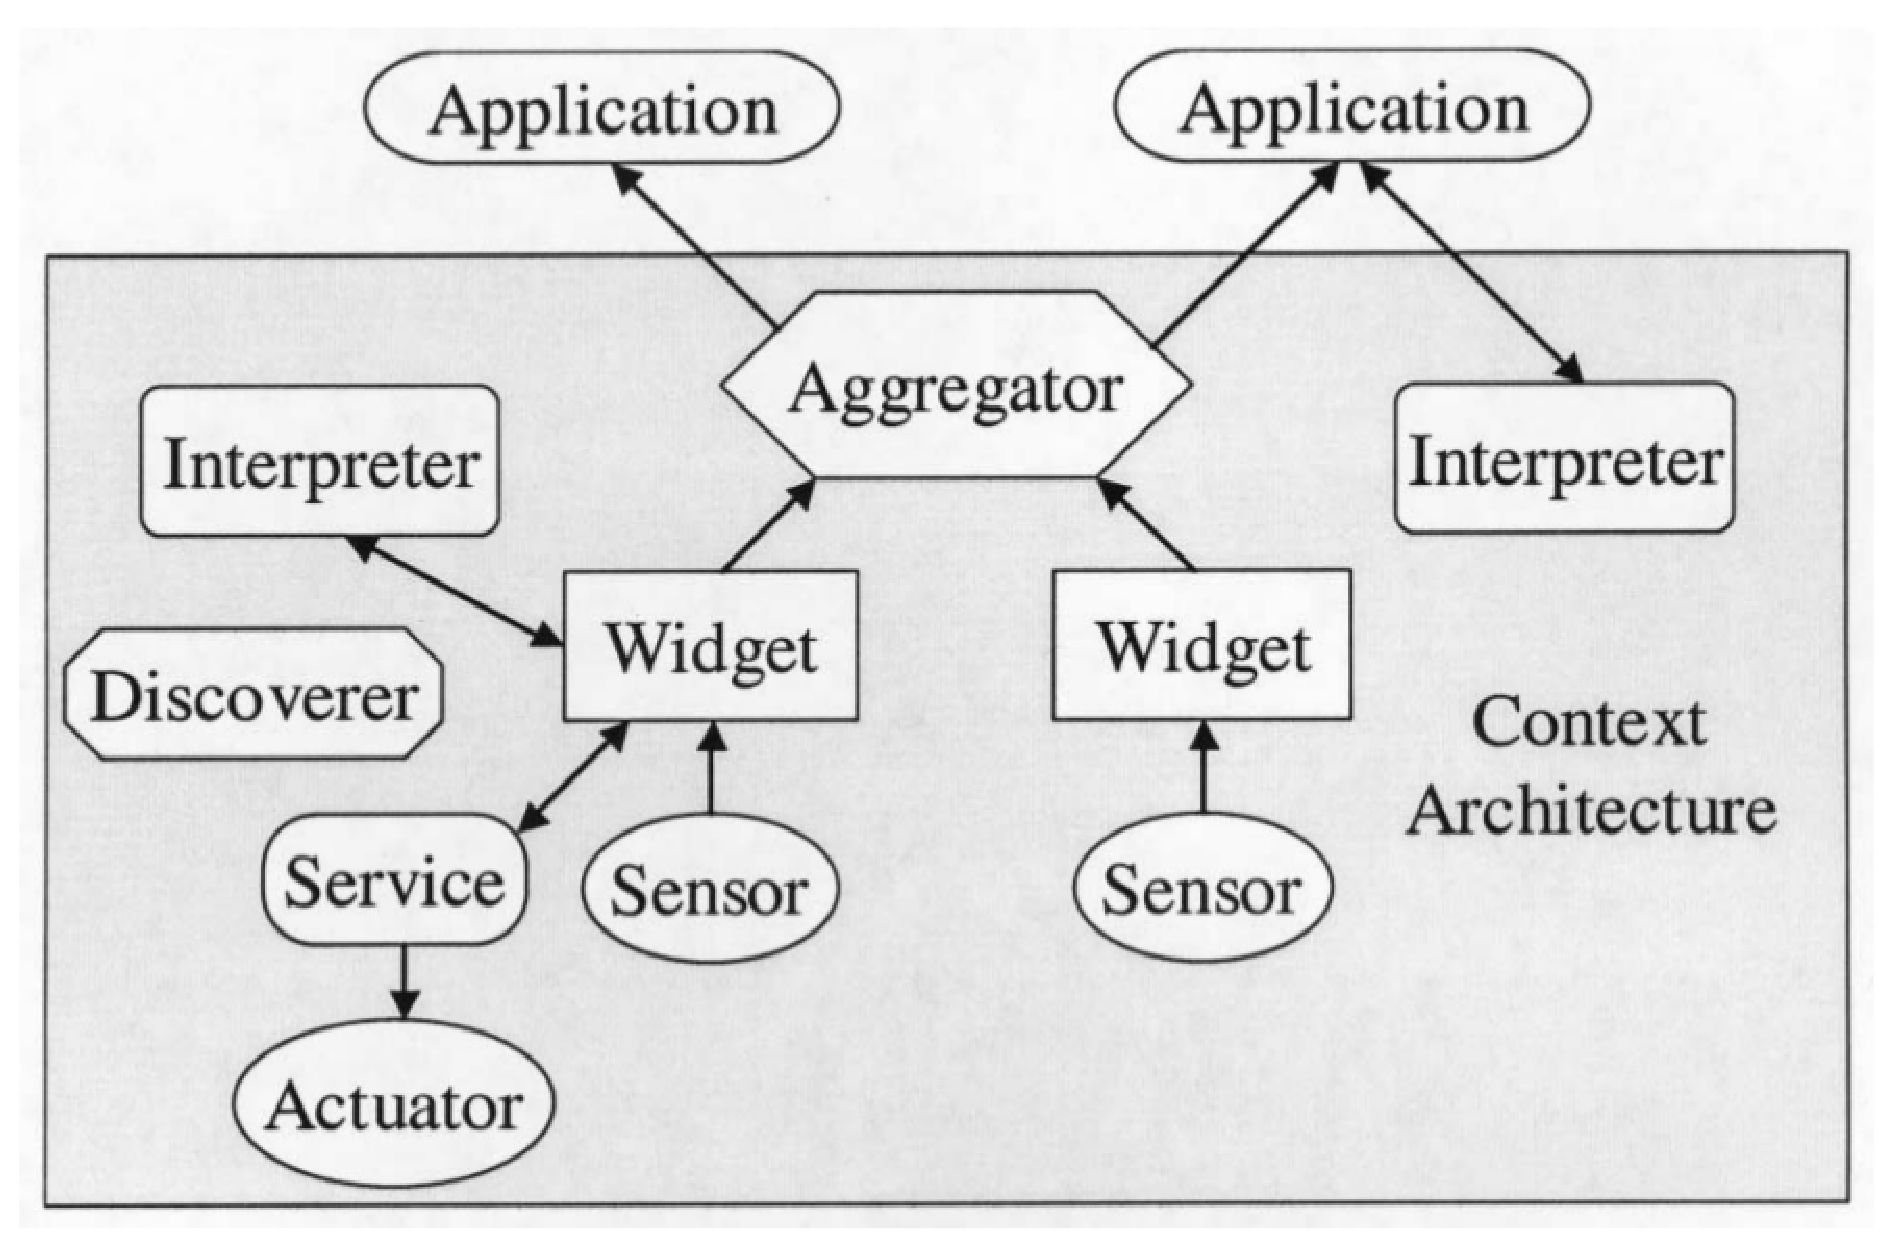
\includegraphics[width=0.6\linewidth]{img/context_toolkit.eps}}
\caption{Example configuration of context toolkit components}
\label{Contexttoolkit}
\end{figure}

\section{Research directions}

Challenges

\section{Conclusion and discussion}

%-------------------------------------------------------------------------------
%	MATERIALS AND METHODS
%-------------------------------------------------------------------------------

%% Optional Materials and Methods Section
%% The Materials and Methods section header will be added automatically.
%
%\begin{materials}
%Suspendisse viverra eleifend nulla at facilisis. Nullam eget tellus orci. Cras
%sit amet lorem velit. Maecenas rhoncus pellentesque orci eget vulputate.
%Phasellus massa nisi, mattis nec elementum accumsan, blandit non neque. In ac
%enim elit, sit amet luctus ante. Cras feugiat commodo lectus, vitae convallis
%dui sagittis id. In in tellus lacus, sed lobortis eros. Phasellus sit amet
%eleifend velit. Duis ornare dapibus porttitor. Maecenas eros velit, dignissim
%at egestas in, tincidunt lacinia erat. Proin elementum mi vel lectus suscipit
%fringilla. Mauris justo est, ullamcorper in rutrum interdum, accumsan eget mi.
%Maecenas ut massa aliquet purus eleifend vehicula in a nisi. Fusce molestie
%cursus lacinia.
%
%\begin{definition}
%A bounded function $\theta$ is a weak solution of QG if for any
%$\phi\,\epsilon\,
%C_0^{\infty}(\fdb\times\mathbb{R}\times[0,\vep])$ we have
%\begin{eqnarray}
%&&  \int_{\mathbb{R}^+\times\fd\times\mathbb{R}} \hspace{-25pt}
% \theta(x,y,t)\, \pr_t \phi
%\,(x,y,t) dy dx dt+\nonumber\\
%  & +&\int_{\mathbb{R}^+\times\fd\times\mathbb{R}}
%\hspace{-26pt} \theta\,(x,y,t) u(x,y,t)\cdot\nabla\phi\,(x,y,t)
%dydxdt = 0 \label{weaksol} \end{eqnarray}
%where $u$ is determined previously.
%\end{definition}
%
%Vestibulum ante ipsum primis in faucibus orci luctus et ultrices posuere
%cubilia Curae; Mauris eu sapien nunc, sit amet accumsan dui. Nulla ac diam ut
%nunc placerat semper eget et libero. Vestibulum ante ipsum primis in faucibus
%orci luctus et ultrices posuere cubilia Curae; Cras hendrerit ullamcorper
%sapien vitae luctus. Quisque vel diam massa. Vestibulum dui nibh, facilisis vel
%vestibulum eu, viverra in quam.
%
%\begin{theorem}
%If the active scalar $\theta$ satisfies
%the equation \eqref{weaksol}, then $\varphi$ satisfies the equation
%\begin{eqnarray}
%\mfrac{\pr \varphi}{\pr t}(x,t)&=&\hspace{-2pt}\dst
%\int_{\fd}\mfrac{\mfrac{\pr \varphi}{\pr x}(x,t)-\mfrac{\pr
%\varphi}{\pr
%u}(u,t)}{[(x-u)^{2}+(\varphi(x,t)-\varphi(u,t))^{2}]^{\f12}}\nonumber\\
%&&
%\chi(x-u,\varphi(x,t)-\varphi(u,t)) du \hspace{3pt} +
%\nonumber\\
%&+&\dst \int_{\fd} \Big{[}\mfrac{\pr \varphi} {\pr
%x}(x,t)-\mfrac{\pr \varphi}{\pr u} (u,t)\Big{]}
%\nonumber\\&&
%\eta(x-u,\varphi(x,t)-\varphi(u,t)) du + Error
%\end{eqnarray}
%with $|Error|\leq C\, \delta | log\delta| $ where $C$ depends only
%on $\|\theta\|_{L^{\infty}}$ and $\|
%\nabla\varphi\|_{L^{\infty}}$.
%\end{theorem}
%
%Class aptent taciti sociosqu ad litora torquent per conubia nostra, per
%inceptos himenaeos. Integer accumsan ornare tortor at varius. Phasellus
%ullamcorper blandit dolor sit amet tempus. Curabitur ligula urna, ultrices in
%iaculis eu, eleifend vel urna. Praesent ullamcorper imperdiet purus, ut
%interdum sem interdum dictum. Proin euismod volutpat eros ac mattis. Quisque
%sit amet massa ac tortor cursus malesuada at vitae nisi. Nam quis neque et nunc
%vehicula cursus sit amet at tellus.
%\end{materials}
%
%-------------------------------------------------------------------------------
%	APPENDICES (OPTIONAL)
%-------------------------------------------------------------------------------

\appendix
An appendix without a title.

\appendix[Appendix title]
An appendix with a title.

%-------------------------------------------------------------------------------
%	ACKNOWLEDGEMENTS
%-------------------------------------------------------------------------------

\begin{acknowledgments}
  Bla bla bla thank you
\end{acknowledgments}


%-------------------------------------------------------------------------------
%	BIBLIOGRAPHY
%-------------------------------------------------------------------------------

%% PNAS does not support submission of supporting .tex files such as BibTeX.
%% Instead all references must be included in the article .tex document. 
%% If you currently use BibTeX, your bibliography is formed because the 
%% command \verb+\bibliography{}+ brings the <filename>.bbl file into your
%% .tex document. To conform to PNAS requirements, copy the reference listings
%% from your .bbl file and add them to the article .tex file, using the
%% bibliography environment described above.  

%%  Contact pnas@nas.edu if you need assistance with your
%%  bibliography.

% Sample bibliography item in PNAS format:
%% \bibitem{in-text reference} comma-separated author names up to 5,
%% for more than 5 authors use first author last name et al. (year published)
%% article title  {\it Journal Name} volume #: start page-end page.
%% ie,
% \bibitem{Neuhaus} Neuhaus J-M, Sitcher L, Meins F, Jr, Boller T (1991) 
% A short C-terminal sequence is necessary and sufficient for the
% targeting of chitinases to the plant vacuole. 
% {\it Proc Natl Acad Sci USA} 88:10362-10366.


%% Enter the largest bibliography number in the facing curly brackets
%% following \begin{thebibliography}

\nocite{*}

\bibliography{biblio}{}
\bibliographystyle{plain}


%\begin{thebibliography}{10}
%\bibitem{BN}
%N.~Gui, H.~Sun V.~De Florio, and C.~Vincenzo Blondia, 
%{\em Toward architecture-based context-aware deployment and adaptationn}, 
%Advances in NIPS, 15 (2003).
%
%\bibitem{BBG:EmbeddingRiemannianManifoldHeatKernel}
%P.~B\'erard, G.~Besson, and S.~Gallot, {\em Embedding {R}iemannian
%  manifolds by their heat kernel}, Geom. and Fun. Anal., 4 (1994),
%  pp.~374--398.
%
%\bibitem{CLAcha1}
%R.R.~Coifman and S.~Lafon, {\em Diffusion maps}, Appl. Comp. Harm. Anal.,
%  21 (2006), pp.~5--30.
%
%\bibitem{DiffusionPNAS}
%R.R.~Coifman, S.~Lafon, A.~Lee, M.~Maggioni, B.~Nadler, F.~Warner, and
%  S.~Zucker, {\em Geometric diffusions as a tool for harmonic analysis and
%  structure definition of data. {P}art {I}: Diffusion maps}, Proc. of Nat.
%  Acad. Sci.,  (2005), pp.~7426--7431.
%
%\bibitem{Clementi:LowDimensionaFreeEnergyLandscapesProteinFolding}
%P.~Das, M.~Moll, H.~Stamati, L.~Kavraki, and C.~Clementi, {\em
%  Low-dimensional, free-energy landscapes of protein-folding reactions by
%  nonlinear dimensionality reduction}, P.N.A.S., 103 (2006), pp.~9885--9890.
%
%\bibitem{DoGri}
%D.~Donoho and C.~Grimes, {\em Hessian eigenmaps: new locally linear
%  embedding techniques for high-dimensional data}, Proceedings of the National
%  Academy of Sciences, 100 (2003), pp.~5591--5596.
%
%\bibitem{DoGri:WhenDoesIsoMap}
%D.~L. Donoho and C.~Grimes, {\em When does isomap recover natural
%  parameterization of families of articulated images?}, Tech. Report Tech. Rep.
%  2002-27, Department of Statistics, Stanford University, August 2002.
%
%\bibitem{GruterWidman:GreenFunction}
%M.~Gr\"uter and K.-O. Widman, {\em The {G}reen function for uniformly
%  elliptic equations}, Man. Math., 37 (1982), pp.~303--342.
%
%\bibitem{Simon:NeumannEssentialSpectrum}
%R.~Hempel, L.~Seco, and B.~Simon, {\em The essential spectrum of neumann
%  laplacians on some bounded singular domains}, 1991.
%
%\bibitem{1}
%Kadison, R.\ V.\ and Singer, I.\ M.\ (1959)
%Extensions of pure states, {\it Amer.\ J.\ Math.\ \bf
%81}, 383-400.
%
%\bibitem{2}
%Anderson, J.\ (1981) A conjecture concerning the pure states of
%$B(H)$ and a related theorem. in {\it Topics in Modern Operator
%Theory}, Birkha\"user, pp.\ 27-43.
%
%\bibitem{3}
%Anderson, J.\ (1979) Extreme points in sets of
%positive linear maps on $B(H)$. {\it J.\ Funct.\
%Anal.\
%\bf 31}, 195-217.
%
%\bibitem{4}
%Anderson, J.\ (1979) Pathology in the Calkin algebra. {\it J.\
%Operator Theory \bf 2}, 159-167.
%
%\bibitem{5}
%Johnson, B.\ E.\ and Parrott, S.\ K.\ (1972) Operators commuting
%with a von Neumann algebra modulo the set of compact operators.
%{\it J.\ Funct.\ Anal.\ \bf 11}, 39-61.
%
%\bibitem{6}
%Akemann, C.\ and Weaver, N.\ (2004) Consistency of a
%counterexample to Naimark's problem. {\it Proc.\ Nat.\ Acad.\
%Sci.\ USA \bf 101}, 7522-7525.
%
%\bibitem{TSL}
%J.~Tenenbaum, V.~de~Silva, and J.~Langford, {\em A global geometric
%  framework for nonlinear dimensionality reduction}, Science, 290 (2000),
%  pp.~2319--2323.
%
%\bibitem{ZhaZha}
%Z.~Zhang and H.~Zha, {\em Principal manifolds and nonlinear dimension
%  reduction via local tangent space alignement}, Tech. Report CSE-02-019,
%  Department of computer science and engineering, Pennsylvania State
%  University, 2002.
%\end{thebibliography}

%-------------------------------------------------------------------------------

\end{article}

%-------------------------------------------------------------------------------
%	FIGURES AND TABLES
%-------------------------------------------------------------------------------

%% Adding Figure and Table References
%% Be sure to add figures and tables after \end{article}
%% and before \end{document}

%% For figures, put the caption below the illustration.
%%
%% \begin{figure}
%% \caption{Almost Sharp Front}\label{afoto}
%% \end{figure}

%\begin{figure}[h]
%\centerline{\includegraphics[width=0.4\linewidth]{placeholder.jpg}}
%\caption{Figure caption}\label{placeholder}
%\end{figure}

%% For Tables, put caption above table
%%
%% Table caption should start with a capital letter, continue with lower case
%% and not have a period at the end
%% Using @{\vrule height ?? depth ?? width0pt} in the tabular preamble will
%% keep that much space between every line in the table.

%% \begin{table}
%% \caption{Repeat length of longer allele by age of onset class}
%% \begin{tabular}{@{\vrule height 10.5pt depth4pt  width0pt}lrcccc}
%% table text
%% \end{tabular}
%% \end{table}

%\begin{table}[h]
%\caption{Table caption}\label{sampletable}
%\begin{tabular}{l l l}
%\hline
%\textbf{Treatments} & \textbf{Response 1} & \textbf{Response 2}\\
%\hline
%Treatment 1 & 0.0003262 & 0.562 \\
%Treatment 2 & 0.0015681 & 0.910 \\
%Treatment 3 & 0.0009271 & 0.296 \\
%\hline
%\end{tabular}
%\end{table}

%% For two column figures and tables, use the following:

%% \begin{figure*}
%% \caption{Almost Sharp Front}\label{afoto}
%% \end{figure*}

%% \begin{table*}
%% \caption{Repeat length of longer allele by age of onset class}
%% \begin{tabular}{ccc}
%% table text
%% \end{tabular}
%% \end{table*}

%-------------------------------------------------------------------------------

\end{document}
